\documentclass[dvipsnames, tikz]{standalone}
\usepackage{amsmath}
\usepackage{arevmath}
\usepackage{xcolor}
\usepackage{tikz}
\usetikzlibrary{calc}
\usetikzlibrary{decorations.pathreplacing,calligraphy,3d}
\usepackage{cmbright}      % sansfont
\usetikzlibrary {arrows.meta} 

\tikzset{main/.style={draw=black, circle, color=black, node distance=5cm, inner sep=0pt,minimum size=1pt}}

\begin{document}
	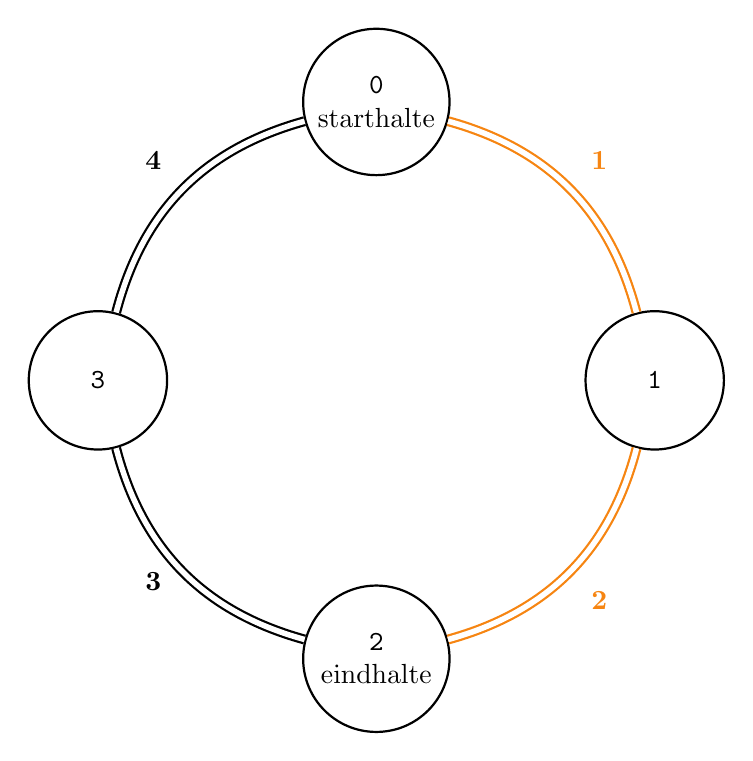
\begin{tikzpicture}[main, line join=bevel]
		\node[thick, main] (A) at (0,0) {\parbox{1.75cm}{\centering \texttt{0}\\starthalte}}; 
		\node[thick, main] (B) [below right of=A]  {\parbox{1.75cm}{\centering \texttt{1}}}; 
		\node[thick, main] (C) [below left of=B] {\parbox{1.75cm}{\centering \texttt{2}\\ eindhalte}}; 
		\node[thick, main] (D) [above left of=C] {\parbox{1.75cm}{\centering \texttt{3}}}; 
		
		\draw [thick, main, BurntOrange] (A) edge[bend left, double, double distance = 2pt] node [above right, xshift=0.25cm, yshift=0.25cm] {\textbf{1}} (B); 
		\draw [thick, main, BurntOrange] (B) edge[bend left, double, double distance = 2pt] node [below right, xshift=0.25cm, yshift=-0.25cm] {\textbf{2}} (C); 
		\draw [thick, main] (C) edge[bend left, double, double distance = 2pt] node [above left, xshift=-0.25cm, yshift=-0.25cm] {\textbf{3}} (D); 
		\draw [thick, main] (D) edge[bend left, double, double distance = 2pt] node [above left, xshift=-0.25cm, yshift=0.25cm] {\textbf{4}} (A); 
	\end{tikzpicture}
\end{document}
